%=============================================================================%
% Preamble
%=============================================================================%
% Libraries

\documentclass[xcolor=table]{beamer}
%\usepackage{beamerthemeshadow}
\usepackage{helvet}
\usepackage[]{graphicx}
\usepackage{array}
\usepackage{color}
\definecolor{dkgreen}{rgb}{0,0.6,0}
\definecolor{gray}{rgb}{0.5,0.5,0.5}
\definecolor{mauve}{rgb}{0.58,0,0.82}
\definecolor{deepblue}{rgb}{0,0,0.5}
\definecolor{deepred}{rgb}{0.6,0,0}
\definecolor{deepgreen}{rgb}{0,0.5,0}
\definecolor{lightgray}{rgb}{0.92,0.92,0.92}
\usepackage{listings} % to insert code
\usepackage{hyperref}
\hypersetup{colorlinks=true, urlcolor=blue, linkcolor=black} 

\lstdefinestyle{bash}{
language=bash,                     % the language of the code
basicstyle=\scriptsize\ttfamily,       % the size of the fonts that are used for the code
numbers=none,%left,                   % where to put the line-numbers
numberstyle=\tiny\color{gray},  % the style that is used for the line-numbers
stepnumber=1,                   % the step between two line-numbers. If it's 1, each line
                          % will be numbered
numbersep=5pt,                  % how far the line-numbers are from the code
backgroundcolor=\color{lightgray},  % choose the background color. You must add \usepackage{color}
showspaces=false,               % show spaces adding particular underscores
showstringspaces=false,         % underline spaces within strings
showtabs=false,                 % show tabs within strings adding particular underscores
frame=lines,%single,                   % adds a frame around the code
rulecolor=\color{black},        % if not set, the frame-color may be changed on line-breaks within not-black text (e.g. commens (green here))
tabsize=2,                      % sets default tabsize to 2 spaces
captionpos=b,                   % sets the caption-position to bottom
breaklines=true,                % sets automatic line breaking
breakatwhitespace=false,        % sets if automatic breaks should only happen at whitespace
title=\lstname,                 % show the filename of files included with \lstinputlisting;
                          % also try caption instead of title
keywordstyle=\color{blue},      % keyword style
commentstyle=\color{dkgreen},   % comment style
stringstyle=\color{mauve},      % string literal style
escapeinside={\%*}{*)},         % if you want to add a comment within your code
morekeywords={}            % if you want to add more keywords to the set
}

\lstdefinestyle{python}{
language=python,
formfeed=\newpage,
basicstyle=\scriptsize\ttfamily,
commentstyle=\color{deepgreen},%\color{gray},
numbers=left,
numberstyle=\tiny\color{gray},
stepnumber=1,
numbersep=5pt,
backgroundcolor=\color{lightgray},%\color{white},
showspaces=false,
showstringspaces=false,
showtabs=false,
frame=lines,
tabsize=4,
captionpos=b,
breaklines=true,
breakatwhitespace=false,
title=\lstname,
escapeinside={},
keywordstyle=\color{deepblue},
emphstyle=\color{deepred},
stringstyle=\color{deepgreen}
%morekeywords={models, lambda, forms}
}

\graphicspath{ {../img/} }

\title{Python for Scientific Research}   
\author{Bram Kuijper}
\institute[]{University of Exeter, Penryn Campus, UK}
\titlegraphic{
\hfill

\includegraphics[width=\textwidth, keepaspectratio]{logo.jpg}}


\begin{document}

\frame{\titlepage} 

\frame{
    \frametitle{Course Schedule} 
    \begin{itemize}
        \item Today, March 6: The basics of programming in Python
            \begin{itemize}
                \item how to run Python code
                \item data types
                \item variable scope
                \item flow control
                \item text manipulation
            \end{itemize}
            \pause
        \item March 20th: Applying Python to simplify your life
            \begin{itemize}
                \item functions
                \item working with files
                \item working with data using \texttt{pandas} and \texttt{scipy}
                \item making graphs using \texttt{matplotlib}
            \end{itemize}
            \pause
        \item March 27th: Advanced subjects
            \begin{itemize}
                \item object-oriented programming
                \item automating tasks in MS-office
                \item image manipulation
                \item working on student-generated problems
            \end{itemize}
    \end{itemize}
}

\frame{
    \frametitle{Today's schedule} 
    \begin{itemize}
        \item 1300 - 1400: How to run Python \& Data types
        \item 1400 - 1420: Break
        \item 1420 - 1520: Variable scope \& Flow control
        \item 1520 - 1540: Break
        \item 1540 - 1640: Functions, working with files 
    \end{itemize}
}

\frame{\frametitle{What is Python?}
\begin{itemize}
    \item A scripted, high-level programming language created by Guido Van Rossum and named after Monty Python's flying circus
\begin{center}
    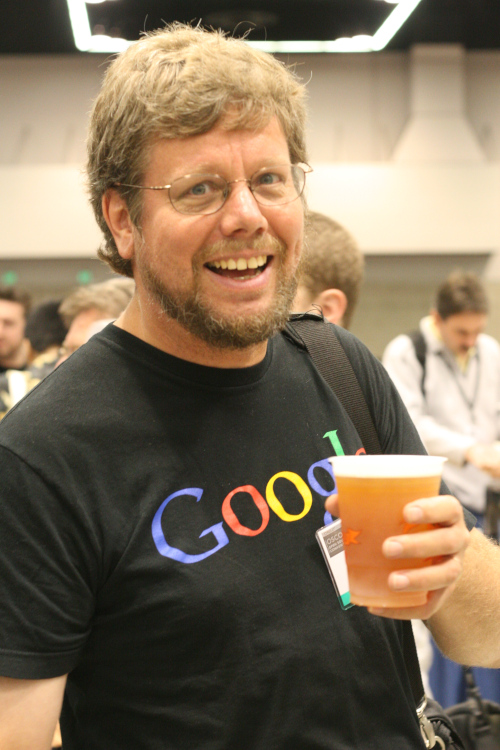
\includegraphics[width = 20mm]{GuidoVanRossumSmall.jpg}
    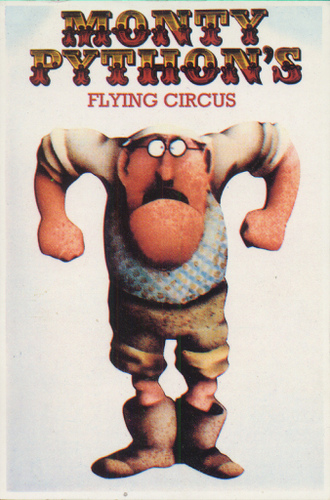
\includegraphics[width = 20mm]{MontyPython.jpg}
\end{center}
    \pause
    \item easy-to-use, highly standardized and with an emphasis on readability of code
\end{itemize}
}


\frame{\frametitle{Why use Python?}
The TIOBE index is a measure of the popularity of programming languages:
    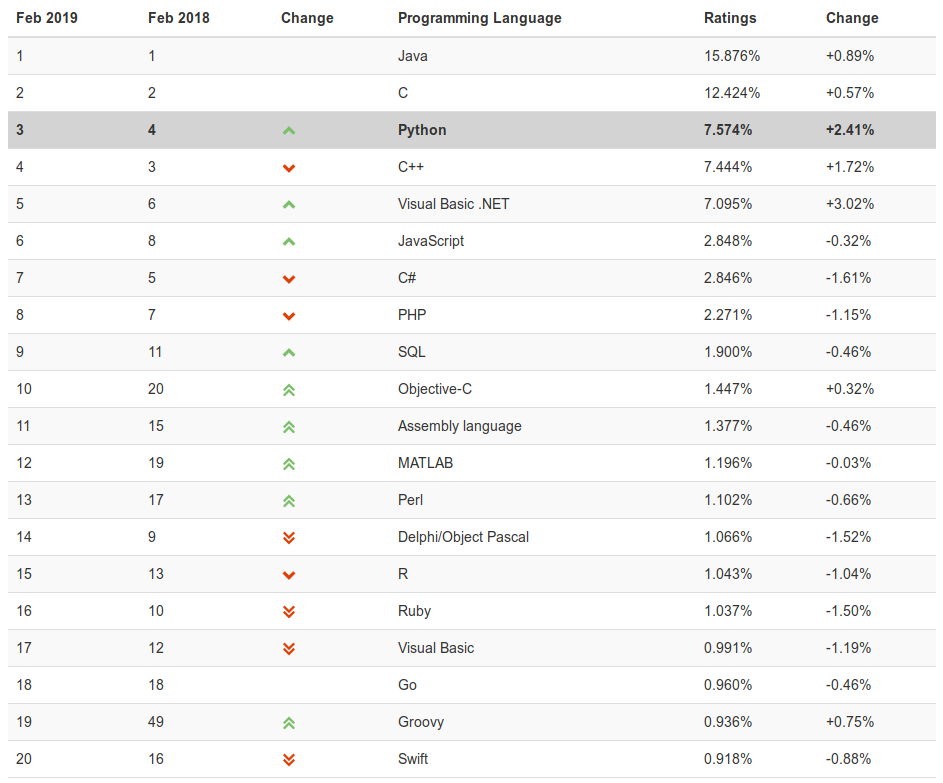
\includegraphics[width = 10cm]{TiobeIndex.png}
}

\begin{frame}{Why Python?}
%. Here are some reasons for its popularity:

\begin{itemize}\addtolength{\itemsep}{0.5\baselineskip}
	\item<1-> It is free! No licence costs
	\item<2-> Runs on all platforms (Mac, Windows, Linux)
	\item<3-> Because of it's ease of programming (e.g no neeed to worry about memory allocation), Python minimises development effort
	\item<4-> A huge number of \href{https://pypi.python.org/pypi}{libraries}, written by an active \href{https://www.python.org/community/}{community}  
	\item<5-> Python can ``glue" together functions written in C/C++ and Fortran to speed things up (we can also call R and MATLAB functions)
	\item<6-> Compared to other high-level scientific languages such as MATLAB and R, Python offers a much wider range of additional functionality (e.g \href{https://www.djangoproject.com/}{web} and \href{https://wiki.python.org/moin/TkInter}{GUI} development) %hence the nickname ``the swiss army knife" of programming languages. 
\end{itemize}

\end{frame}

\frame{\frametitle{Python compared to other languages}
\rowcolors{1}{}{lightgray}
\begin{tabular}{c c c c c}
    & Python & C/C++ & Java & R 
\pause 
    \\ 
    Speed & Slow & Fast & OK & Very Slow \pause \\  
    Easy to code? & Very easy & Hard & Hard/OK & OK \pause \\  
    Easy to port? & Very easy & Hard & Very easy & Easy \pause \\  
    Documentation & Excellent & Very poor & Poor & Poor \pause \\  
\end{tabular}
}


\frame{\frametitle{Tables with pause}
\begin{tabular}{c c c}
A & B & C \\ 
\pause 
1 & 2 & 3 \\  
\pause 
A & B & C \\ 
\end{tabular} }

\frame{\frametitle{blocs}

\begin{block}{title of the bloc}
bloc text
\end{block}

\begin{exampleblock}{title of the bloc}
bloc text
\end{exampleblock}


\begin{alertblock}{title of the bloc}
bloc text
\end{alertblock}
}
\end{document}

